\documentclass[a4paper, 11pt]{article}
\usepackage{comment}
\usepackage{fullpage}
\usepackage{amsmath}
\usepackage{amssymb}
\usepackage{mathtools}
\usepackage{fontspec}
\usepackage{siunitx}
\defaultfontfeatures{Ligatures=TeX}
\usepackage{xfrac}
\usepackage{icomma}
\usepackage[section,below]{placeins}
\usepackage[labelfont=bf,font=small,width=0.9\textwidth]{caption}
\usepackage{subcaption}
\usepackage{graphicx}
\usepackage{grffile}
\usepackage{float}
\floatplacement{figure}{htbp}
\floatplacement{table}{htbp}
\usepackage{booktabs}
\usepackage{hyperref}
\begin{document}
\noindent
\centerline{\small{\textsc{Michigan State University}}} \\
\large{\textbf{CMSE/CSE 822 – Parallel Computing \hfill Fall 2019 \\
Homework 3}} \\
Alexander Harnisch \\
\noindent\makebox[\linewidth]{\rule{\textwidth}{0.4pt}}

\section*{1) Compilers and auto-vectorization}
\subsection*{a.}
\label{sec:1a}
The Intel16 system's CPU used here is a Xeon E6-2680 by Intel, running at a
clock speed of \SI{2.4}{\giga\hertz}. Figure~\ref{fig:cache_table} shows the
cache size and layout. However, the processor supports turbo boosting at
\SI{3.3}{\giga\hertz} for a single core and \SI{2.9}{\giga\hertz} for all 14
cores at once. The CPU has 14 physical cores with Intel's hyper-threading
technology, effectively having 24 virtual cores or simultaneous threads.
Assuming the processor is capable of one floating point operation per clock
cycle and thread running at \SI{2.9}{\giga\hertz} turbo boost, the theoretical
peak performance would be \SI{96.6}{\giga FLOP \per\second}. However, the
assignment is not precise enough to know what exactly it is asking for. Single
thread performance? Turbo boost yes or no? The theoretical single thread peak
performance at a boosted clock frequency of \SI{3.3}{\giga\hertz} would simply
be \SI{3.3}{\giga FLOP\per\second}. The sustainable single thread peak
performance at \SI{2.4}{\giga\hertz} would be \SI{2.4}{\giga FLOP\per\second}.
Multiply that by 24 for sustainable multithread peak performance. I am tired of
trying to guess what the assignments are asking for.
\begin{figure}
  \centering
  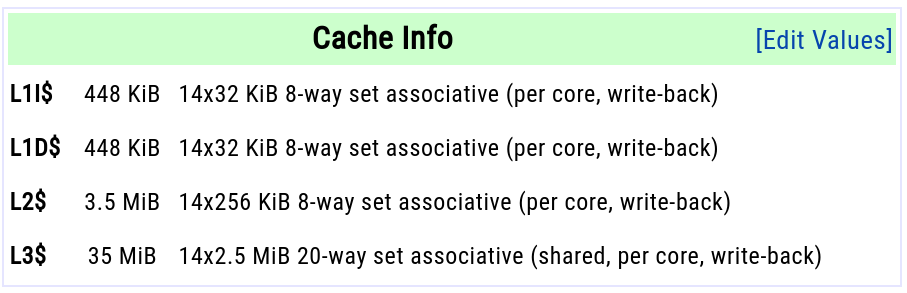
\includegraphics[width=.7\textwidth]{./cache_table.png}
  \caption{Xeon E5-2680 v4 cache size and layout~\cite{wikichip}.}
  \label{fig:cache_table}
\end{figure}

\subsection*{b.}
Again, depends on so many assumptions that have to be made and are not given by
the problem statement. Assuming \SI{32}{bit} single-precision floating point
numbers, AVX can perform the same instructions on up to 8 data streams at a
time. That would mean we get another factor of 8. Additionally, assuming that
all operations are of the type $a+b\times c$ which can be done in one operation
using FMA we get another factor of 2. So we simply take whatever the correct
answer in \hyperref[sec:1a]{1) a.} is supposed to be and multiply it by 16.

\subsection*{c.}
<+Placeholder+>

%%%%%%%%%%%%%%%%%%%%%%%%%%%%%%%%% Bibliography %%%%%%%%%%%%%%%%%%%%%%%%%%%%%%%%
\begin{thebibliography}{9}
  \bibitem{wikichip}
  WikiChip.
  \textit{Xeon E5-2680 v4 - Intel}.
  \href{https://en.wikichip.org/wiki/intel/xeon\_e5/e5-2680\_v4}
  {https://en.wikichip.org/wiki/intel/xeon\_e5/e5-2680\_v4}.
\end{thebibliography}
\end{document}
